\section{Introduction}
{\tiny Written by: Philipp Becker}\\
\subsection{Main Vision}
Our Inventory Management System revolutionizes the way educational institutions manage and rent lockers and devices, promoting efficiency, equality, and sustainability. Users can effortlessly search for and rent lockers to charge their devices or store essential items such as laptops to charge them. Additionally they can rent devices such as drones from the institution's inventory. This system not only simplifies the process for users but also provides administrators with advanced device tracking and comprehensive reporting tools for faulty hardware. These features collectively contribute to a seamless, stress-free experience, enhancing productivity and convenience for all stakeholders.

\subsection{Core Values and Project Goals}
Core values are fundamental principles and beliefs that guide the behavior and decision-making process within an organization. They represent the essence of what the organization stands for and help shape its culture and identity. \\Our chosen core values are \textbf{Sustainability, Equality,} and \textbf{Stressless.} We selected these values because they align with our vision of creating a responsible, inclusive, and user-friendly Inventory Management System.

\begin{enumerate}
\item \textbf{Sustainability:} We aim to incorporate eco-friendly practices in our system, such as promoting the use of energy-efficient devices and reducing waste. Our goal is to ensure that our operations have a positive impact on the environment, contributing to a healthier planet and setting a positive example for others.
\item \textbf{Equality:} We are committed to providing equal access and opportunities for all users, regardless of their background or circumstances. This involves ensuring our system is accessible to everyone, offering fair rental terms, and fostering an inclusive environment. Our goal is to support equal education by making essential tools and resources available to all students.

\item \textbf{Stressless:} Our objective is to create a user-friendly system that minimizes the stress associated with managing and renting equipment. By streamlining processes, offering intuitive interfaces we make it easier for both users and administrators to interact with our system. A stress-free experience enhances satisfaction and productivity for all parties involved.
\end{enumerate}

By adhering to these core values, our project goals focus on achieving a sustainable, equitable, and user-friendly system that meets the needs of all stakeholders.

\subsection{Core Functionalitys}
\subsubsection{Renting Devices and Lockers}
\begin{itemize}
\item \textbf{Renting Devices:} Users can rent devices through an intuitive interface, which allows them to select, reserve, and access devices based on availability and specific needs. The devices available for rent are stored in lockers and can be picked up using a provided access code.
\item \textbf{Renting Lockers:}  The system provides capabilities for users to rent lockers, facilitating a secure and convenient way to store personal devices within the facility. Additionally, users can charge their devices in the rented locker and monitor the wattage flow through the frontend interface.
\end{itemize}

\subsubsection{Managing Devices \& Lockers}
\begin{itemize}
\item \textbf{Manage Devices:} Administrators can create, categorize, and manage devices. They have the ability to oversee all device allocations, track device status, update device information, and view all bookings.

\item \textbf{Manage Lockers:} This feature allows administrators to create and manage lockers and monitor their status. Administrators can also view and manage all locker bookings.
\end{itemize}

\subsubsection{Reporting and Manage Problems}
\begin{itemize}

\item \textbf{Report Problems: }Users can report any issues they encounter with the devices or lockers, such as malfunctions or access problems. The problems, along with all relevant booking information, are sent to the administrator.

\item \textbf{Manage Problems: }Enables the administration to efficiently handle and resolve reported problems related to devices or lockers, improving service quality and user satisfaction.
\end{itemize}

\subsection{Team Composition and Responsibilities}
In this project, members were divided into specific teams based on their interests and expertise. Each team was assigned specific components of the project, ensuring that their distinct expertise contributed to the comprehensive development and integration of the system, while also collaborating effectively to meet the project's overarching goals. This section outlines the team structure, member assignments, and their respective responsibilities. 
\subsection{Team Introduction}
\subsubsection{Jingya Zhao}
Centria University of Applied Sciences \\
Degree Program: Information Technology

\subsubsection{Kandaker Majharul Islam}
Centria University of Applied Sciences \\
Degree Program: Information Technology

\subsubsection{Felix Huther}
Hochschule Darmstadt, University of Applied Sciences \\
Degree Program: Computer Science

\subsubsection{Sven Lepper}
Hochschule Darmstadt, University of Applied Sciences \\
Degree Program: Computer Science

\subsubsection{Philipp Becker}
Hochschule Darmstadt, University of Applied Sciences \\
Degree Program: Computer Science

\subsection{Team grouping and Task allocation}

Each team in our project defined their own set of work packages using ClickUp, a versatile tool designed to manage task-based work through a Kanban board visualization. Afterward, we collaboratively addressed cross-team responsibilities and integration tasks. Every three days, we discussed these tasks together, ensuring continuous alignment with project goals and effective problem-solving.

\begin{figure}[h]
    \centering
    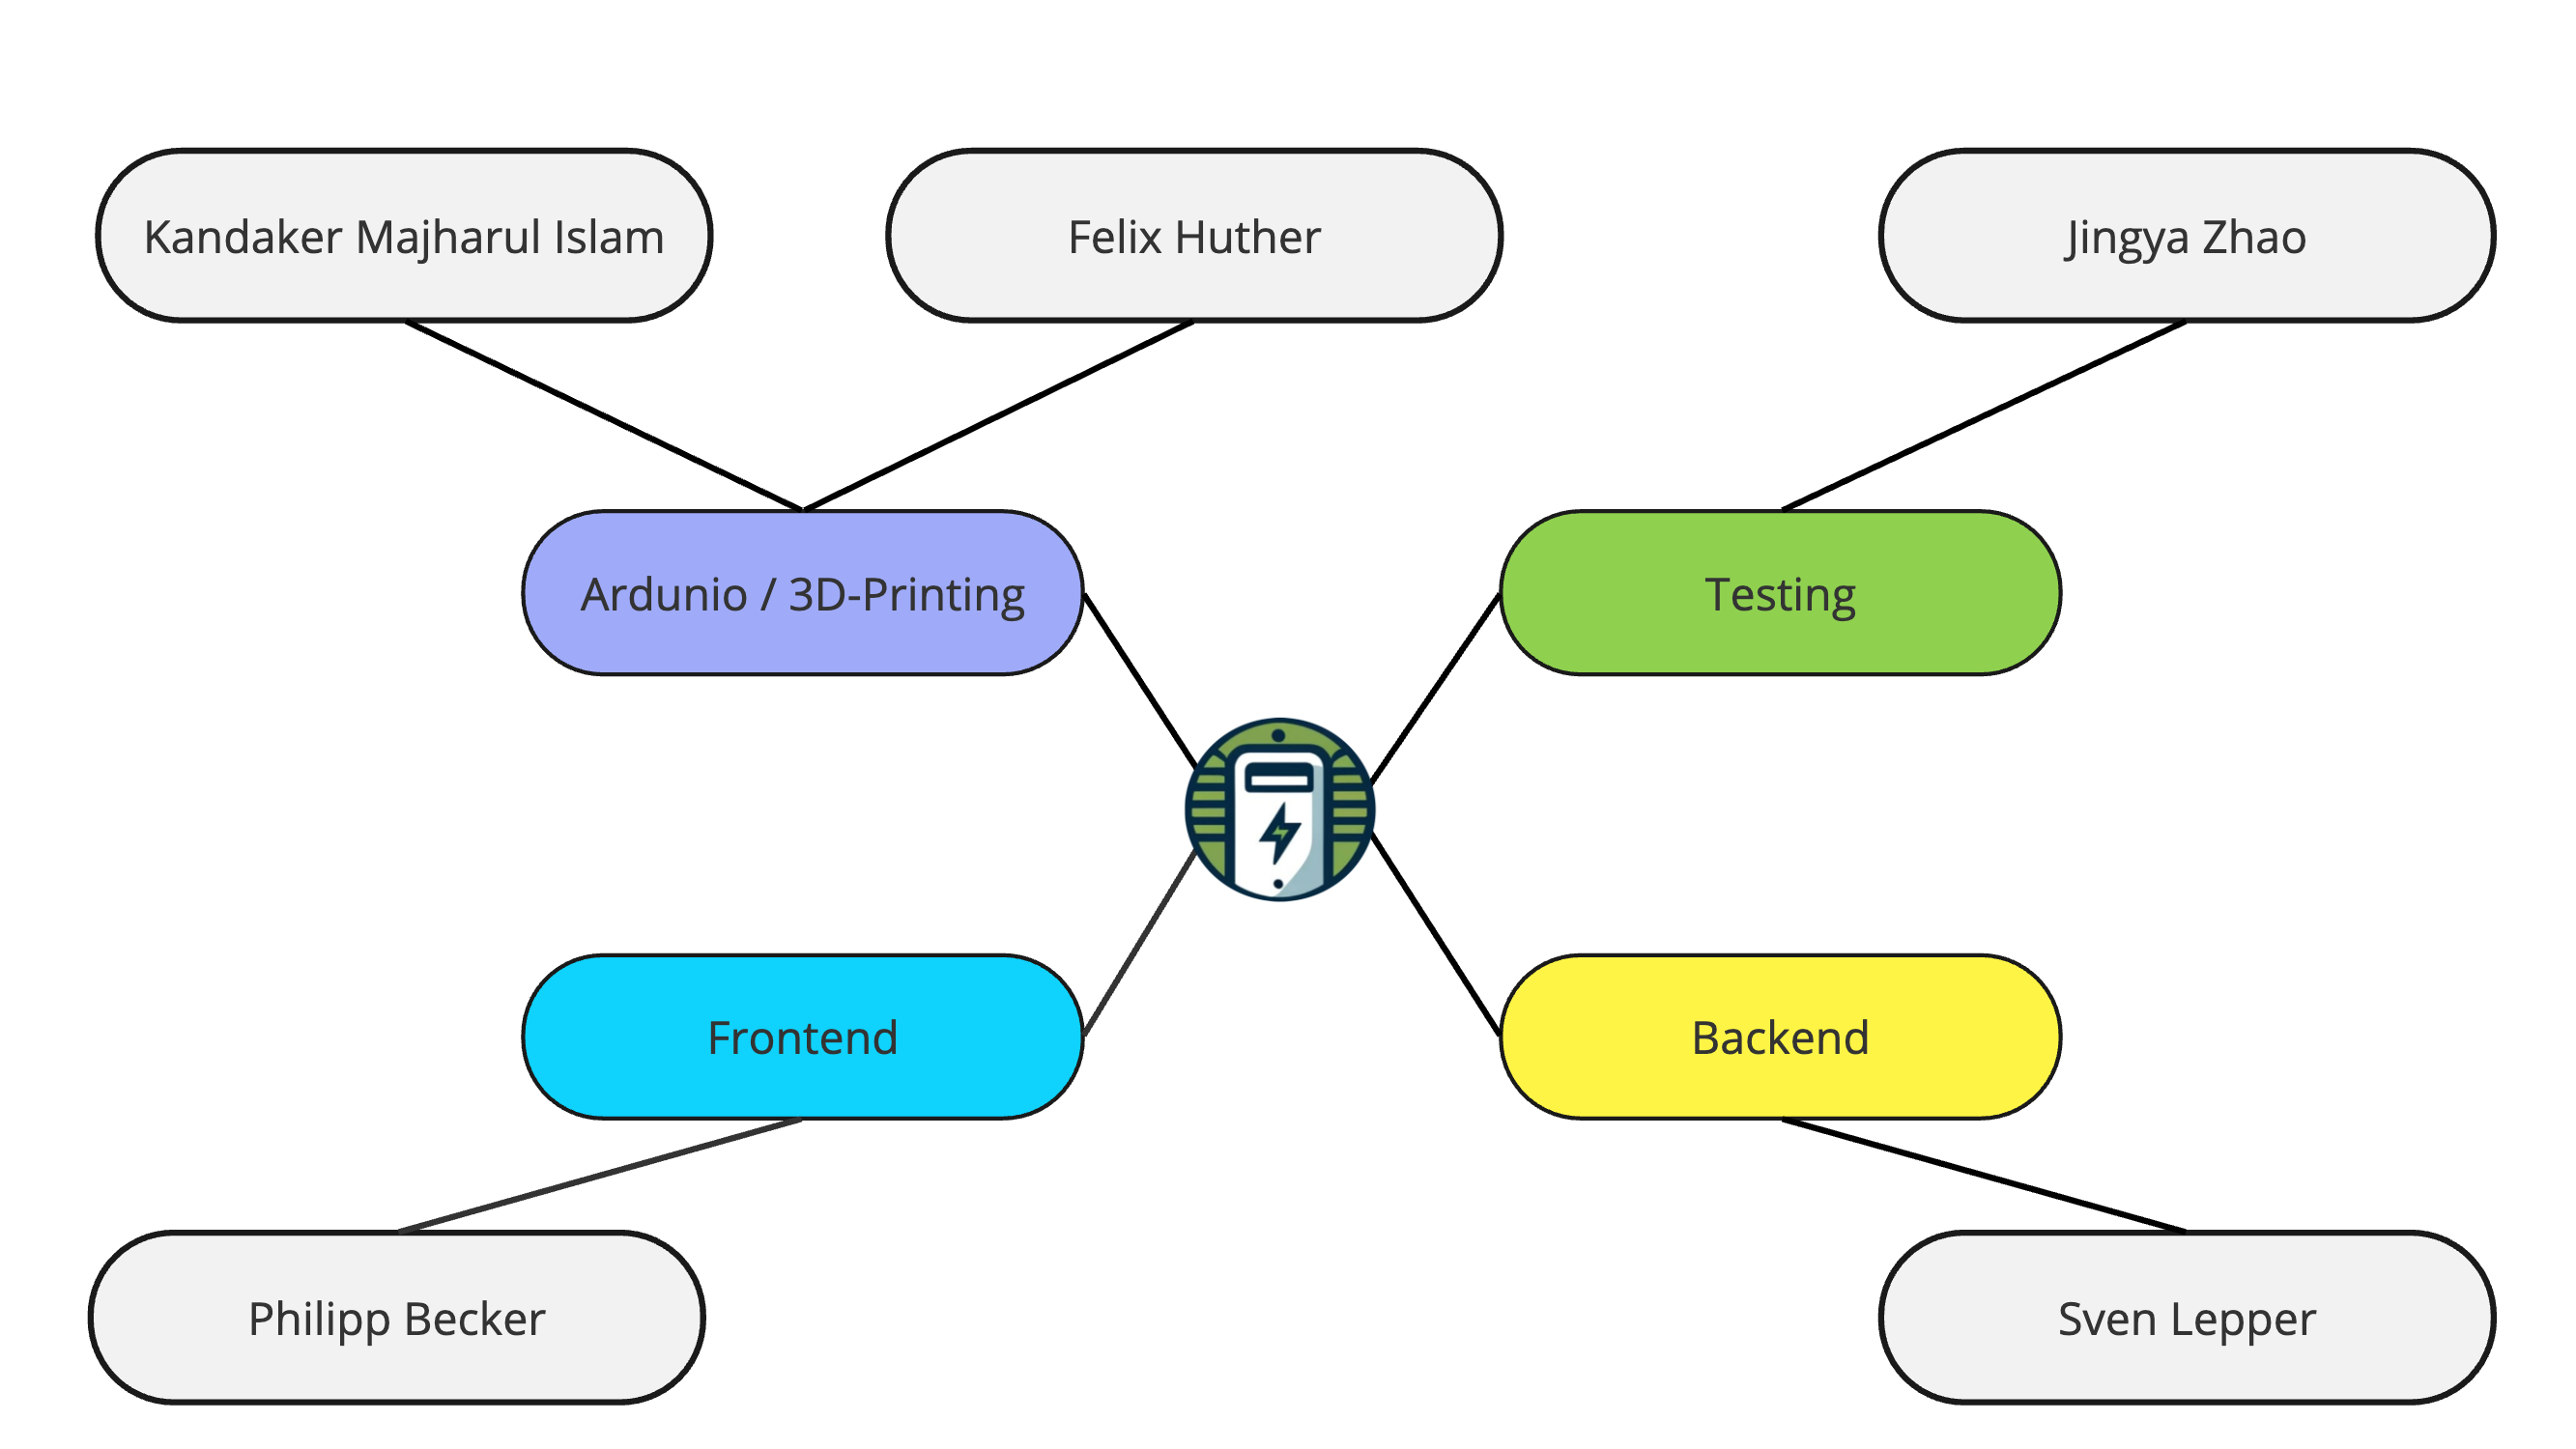
\includegraphics[width=0.8\textwidth]{images/project_split}
    \caption{Team Composition and Responsibilities}
\end{figure}


%Each team in our project independently defined their own set of work packages using ClickUp, a versatile tool designed to manage task-based work through a Kanban board visualization. This approach allowed every team member to clearly see their tasks and responsibilities, facilitating better planning and coordination. To maintain momentum and ensure continuous alignment with project goals, the teams reviewed the board every three days. These meetings served as mini-sprints, akin to the Scrum methodology, where progress was assessed, and adjustments were made as necessary.


\subsubsection{Hardware and 3D Print}
The Hardware and 3D Printing team was led by Felix Huther, with significant assistance from Kandaker Majharul Islam. Felix was primarily responsible for designing the 3D models, overseeing the prototype printing, and managing the hardware assembly. Kandaker supported Felix in all these tasks and was introduced to programming the Arduino device, where he implemented several smaller functions. This team also integrated REST APIs for real-time data transmission, sending live data to the frontend via ThingSpeak and ensuring backend communication.

\begin{figure}[htbp]
    \centering
    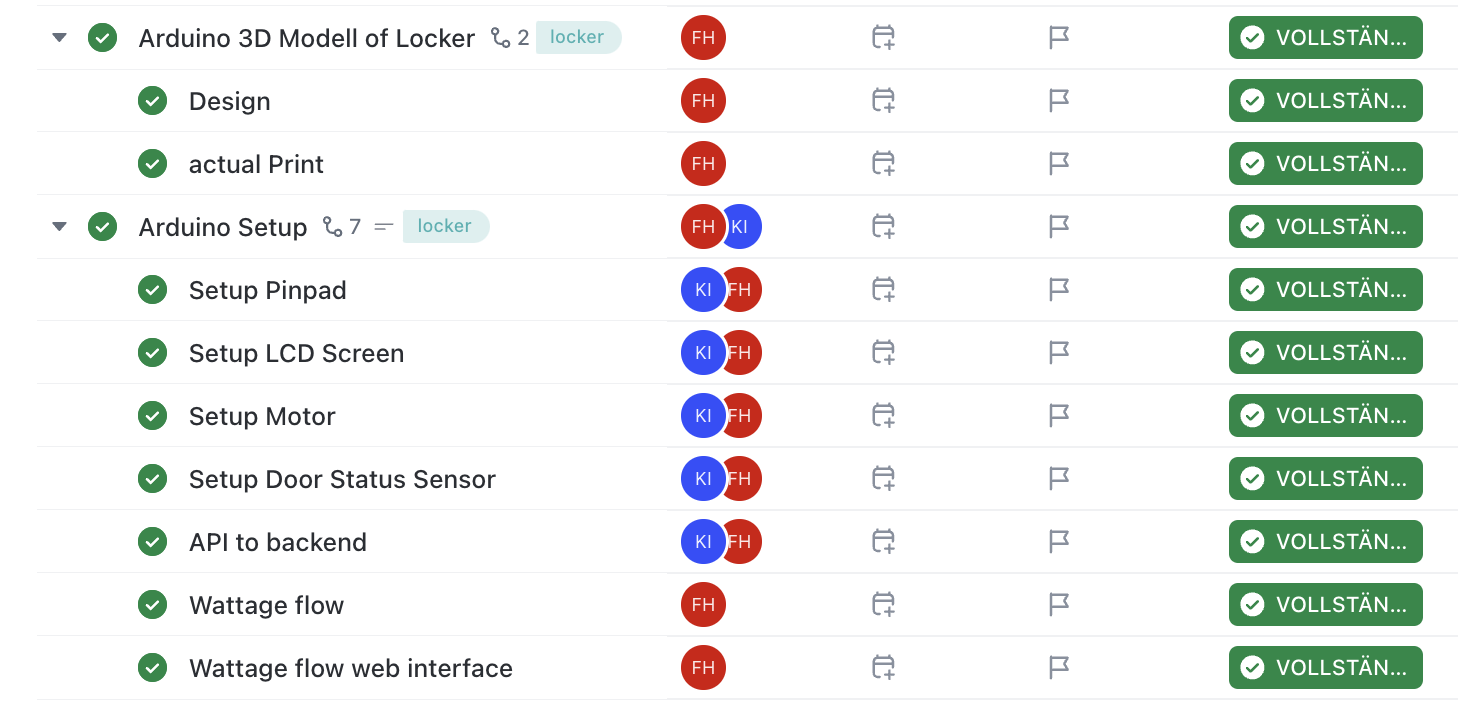
\includegraphics[width=0.9\textwidth]{images/hardware and print.png}
    \caption{Hardware and 3D Model Tasks}
    \label{fig:myimage}
\end{figure}

\subsubsection{Frontend Development}
Philipp Becker was responsible for the Frontend development, utilizing Vue.js in TypeScript, styled with Tailwind CSS and Vue-Bootstrap. This setup facilitated a robust and responsive user interface. Philipp also integrated the Google Maps API to show the current location of the locker on a map. The frontend implementation was split into two tasks: Admin-Frontend for administrative tasks such as management, reports, and bookings, and User-Frontend for locker rentals, device rentals, and problem reporting.

\begin{figure}[htbp]
    \centering
    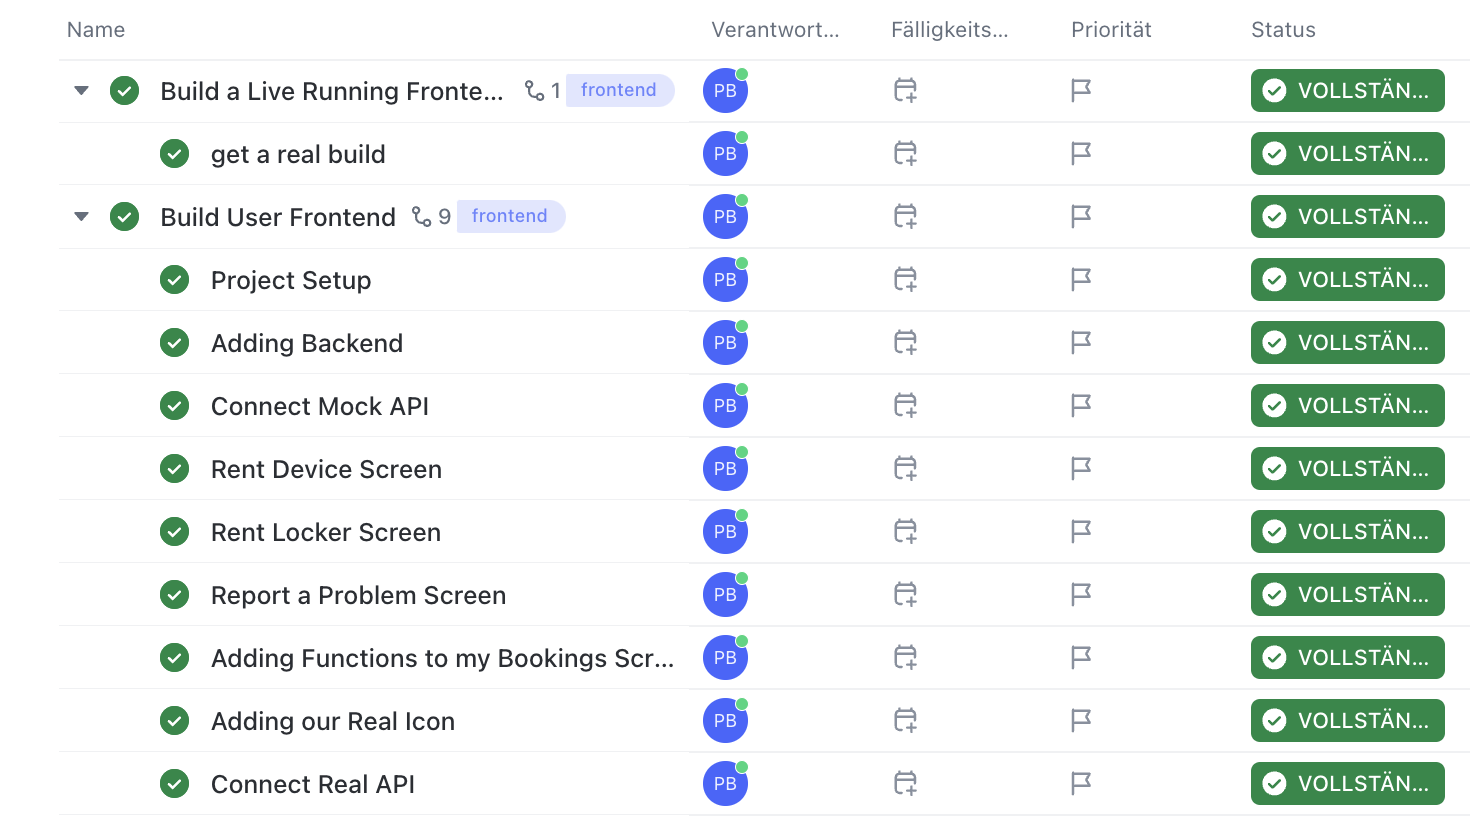
\includegraphics[width=0.9\textwidth]{images/user-frontend.png}
    \caption{User-Frontend Tasks}
    \label{fig:myimage}
    \vspace{1cm}
    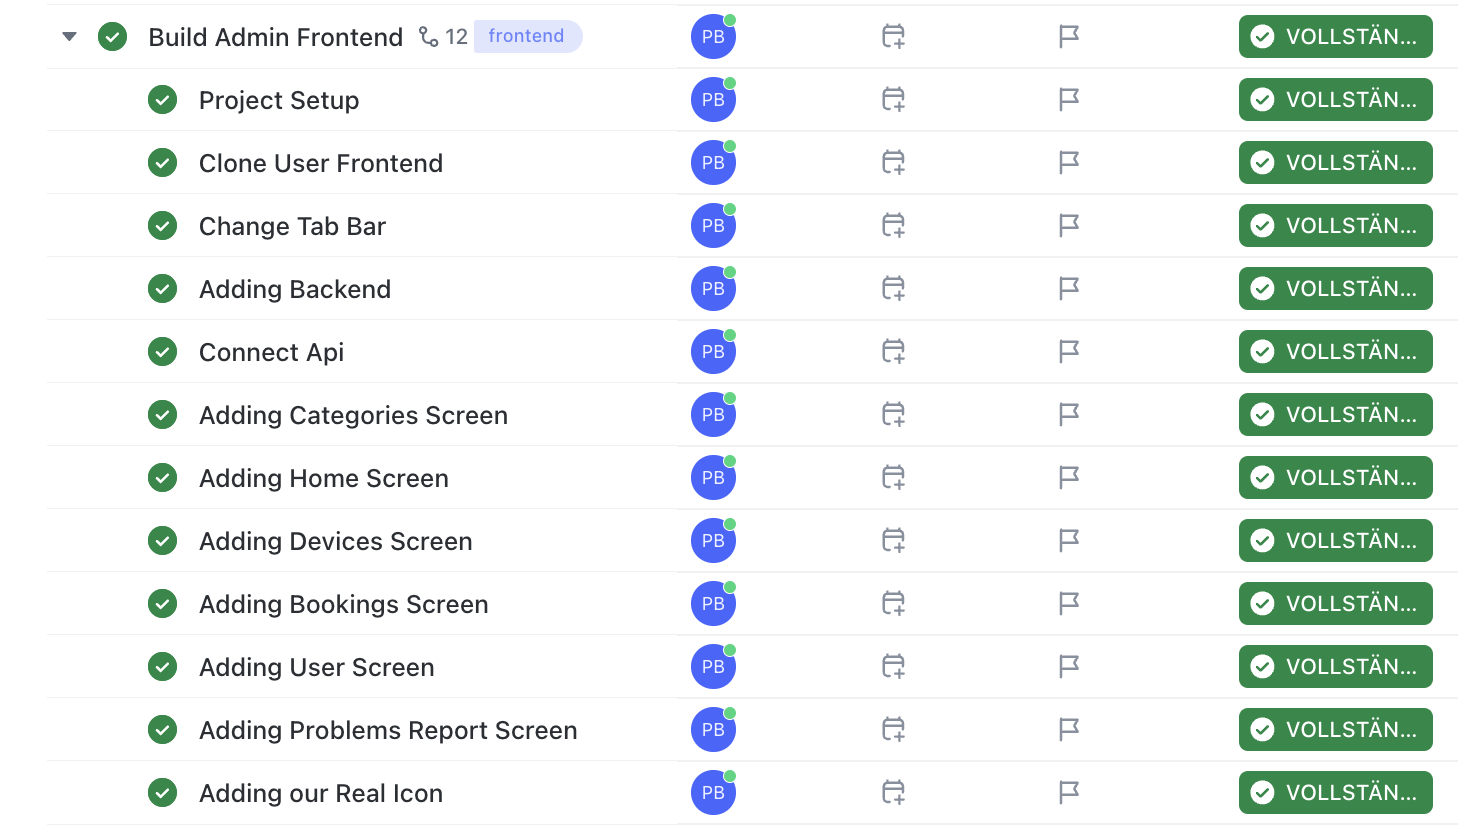
\includegraphics[width=0.8\textwidth]{images/admin-frontend.png}
    \caption{Admin-Frontend Tasks}
    \label{fig:myimage}
\end{figure}
\clearpage
\subsubsection{Backend Development}
Sven Lepper handled Backend development, employing Alembic with SQL Alchemy as the Object-Relational Mapper (ORM) and PostgreSQL for database management. Fast API was used to create a RESTful interface, enabling efficient communication between all components and the database. This setup provided a solid backbone for the application's data handling requirements.

\begin{figure}[h]
    \centering
    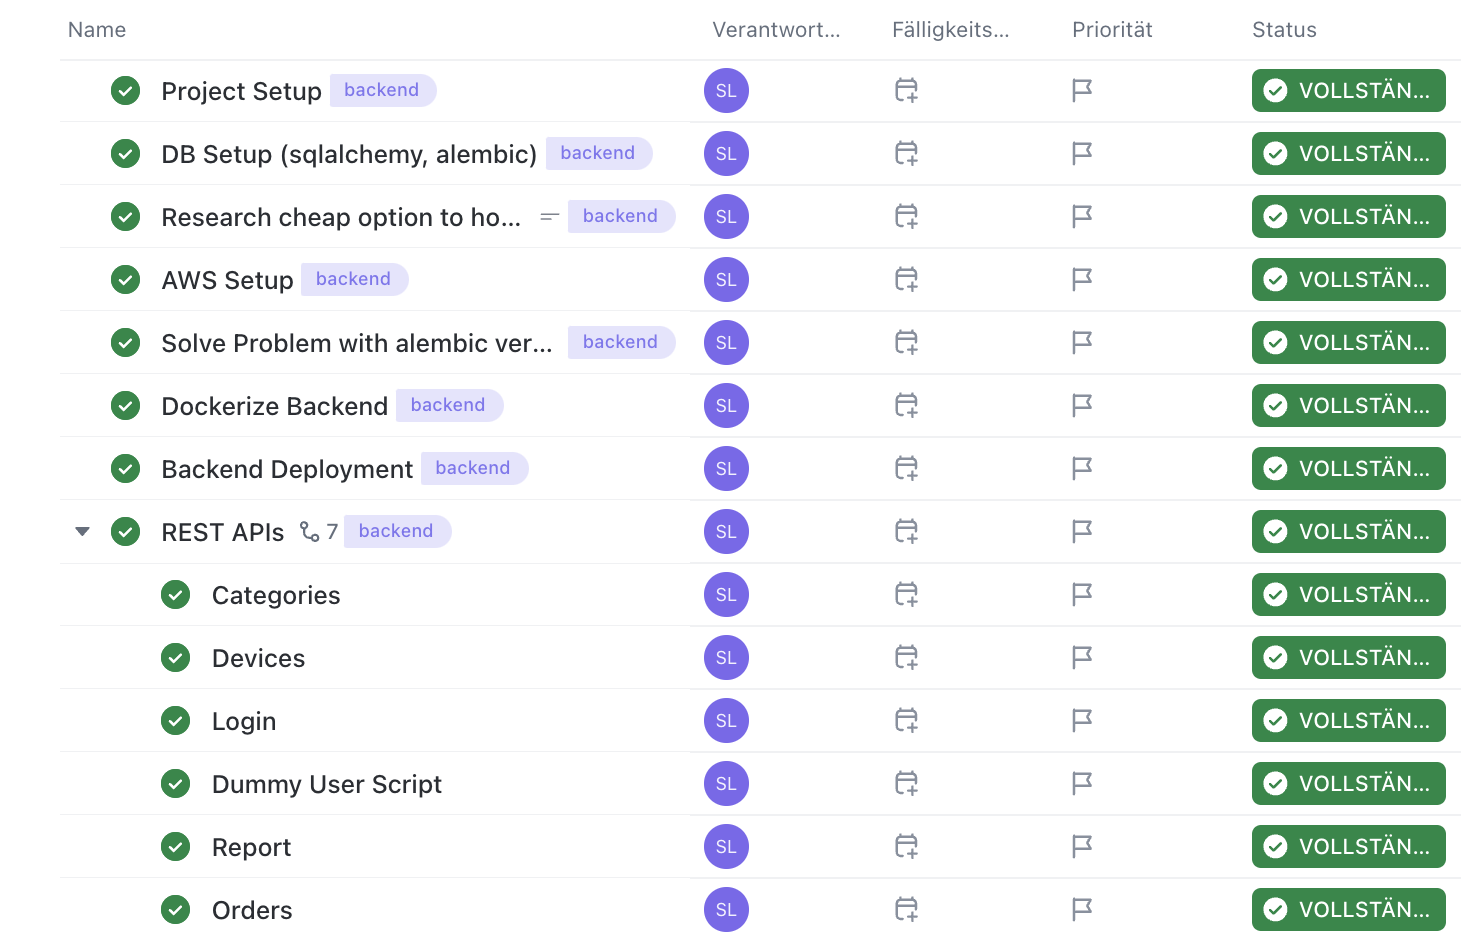
\includegraphics[width=0.9\textwidth]{images/backend.png}
    \caption{User-Frontend Tasks}
    \label{fig:myimage}
\end{figure}
\clearpage
\subsubsection{API Testing and Hardware Research}
Jingya Zhao took charge of API Testing and Hardware Research. She developed automated tests using Postman, which validated the correctness of data across all backend endpoints. Additionally, Jingya conducted research on live tracking technologies for monitoring the energy usage of devices, which was crucial for the real-time data feature in the project.

\begin{figure}[h]
    \centering
    
\includegraphics[width=0.9\textwidth]{images/R&d.png}
    \caption{Hardware Research Tasks}
    \label{fig:myimage}
    \vspace{1cm}
    
\includegraphics[width=0.9\textwidth]{images/testing.png}
    \caption{API Testing Tasks}
    \label{fig:myimage}
\end{figure}

